\documentclass{article}
\usepackage[letterpaper]{geometry}
\geometry{verbose,tmargin=1in,bmargin=1in,lmargin=1in,rmargin=1in}

\usepackage[utf8]{inputenc}
\usepackage{amsmath}
\usepackage{listings}
\usepackage{graphicx}
\usepackage{enumitem}
\usepackage{amssymb}
\usepackage{tabularx}
\usepackage{hyperref}
\usepackage{caption}
\usepackage{float}
\usepackage[section]{placeins}
\usepackage{empheq}
\usepackage{stackengine}
\usepackage{subcaption}
\usepackage{array}

\def\delequal{\mathrel{\ensurestackMath{\stackon[1pt]{=}{\scriptstyle\Delta}}}}


\title{CIS 419/519: Homework 6}
\author{Jiatong Sun}
\date{04/11/2020}

\begin{document}
    \maketitle
    \noindent
    Although the solutions are entirely my own, I consulted with the following people and sources while working on this homework: $Yuchen Sun$\\
    https://pytorch.org/docs/stable/
    
    \section{Reinforcement Learning \uppercase\expandafter{\romannumeral 1}}
    \noindent
    The reward function is fine because for a situation to have a robot run a maze can break down naturally into episodes and thus, simply using the sum of rewards is reasonable.\\\\
    However, if the map is large and the episode length is not long enough, the agent will probably fail to discover the exit for many episodes. After running the agent for a while, the agent may never know there can be a total reward better than 0. Besides, since every policy it has already tried gives the same total reward 0, the agent will have no clue how to choose its policy for the following episode. Therefore, the policy is not improved.\\\\
    There are two easy ways to solve the problem: increase the episode length and/or give non-goal state a value -1. This means the states that have been visited a lot will get worse and worse values so the agent will want to avoid that state. In this way, the agent can eventually reach the goal.
        
    \section{Reinforcement Learning \uppercase\expandafter{\romannumeral 2}}
    According to equation for the expected discount return and value of a state:
    $$R_t=\sum_{k=0}^{\infty}\gamma^kr_{t+k+1}\qquad V^{\pi}(s)=\mathbb{E}[R_t|s_t=s]$$
    If we add a constant $C$ to all the rewards, the total reward changes into
    \begin{equation}\label{eq:reward}
    	\begin{split}
    	R'_t
    	&=\sum_{k=0}^{\infty}\gamma^k(r_{t+k+1}+C)\\
    	&=\sum_{k=0}^{\infty}\gamma^kr_{t+k+1}+\sum_{k=0}^{\infty}\gamma^kC\\
    	&=\sum_{k=0}^{\infty}\gamma^kr_{t+k+1}+\dfrac{C}{1-\gamma} \\
    	&=R_t+\dfrac{C}{1-\gamma}
    	\end{split}
    \end{equation}
    The state value changes into
    \begin{equation}\label{eq:state value}
    	\begin{split}
    	V^{\pi'}(s)
    	&=\mathbb{E}[R_t'|s_t=s]\\
    	&=\mathbb{E}[R_t+\dfrac{C}{1-\gamma}|s_t=s]\\
    	&=\mathbb{E}[R_t|s_t=s]+\dfrac{C}{1-\gamma}\\
    	&=V^{\pi}(s)+\dfrac{C}{1-\gamma}
    	\end{split}
    \end{equation}
    Define $K\delequal\sum_{k=0}^{\infty}\gamma^kC=\dfrac{C}{1-\gamma}$, then $K$ is a constant.\\\\
    \begin{enumerate}
    	\item[(a)]
    	From equation \ref{eq:reward} and equation \ref{eq:state value}, we know that adding a constant to all the rewards only has the effect of shifting the total reward and state value, so the relative reward and relative state value remain the same. \\\\
    	Because we choose the policy that maximize the total reward, we still get the same best policy as before. So \textbf{only the interval between those rewards matters}.\\\\
    	The signs of those rewards are not important. For example, if we change \{+1 for a goal, -1 for a collision\} to \{-1 for a goal, -3 for a collision\}, the best policy gets worse rewards, but it will still be the best policy among all. Changing every reward to negative value essentially means finding a relative better policy among a group of bad policies.
    	\item[(b)]See the proof above.
    	\item[(c)]$K=\sum_{k=0}^{\infty}\gamma^kC=\dfrac{C}{1-\gamma},\; 0<\gamma<1$
    \end{enumerate}
    
    	
    \section{Random policy for the MountainCar gym environment}
    \begin{enumerate}
    	\item[(\romannumeral 1)]
    	action space:\\
    	
		\begin{table}[h]
        \centering
		\begin{tabularx}{0.4\textwidth} { 
 			| >{\centering\arraybackslash}X 
   			| >{\centering\arraybackslash}X | }
 			\hline
 			\textbf{Num} & 
 			\textbf{Action}\\
 			\hline
 			0 & push left\\
 			\hline
 			1 & no push\\
 			\hline
 			2 & push right\\
 			\hline
		\end{tabularx} 
		\label{tab:1}
		\end{table}
		
		observation space:\\
		   
		\begin{table}[h]
        \centering
		\begin{tabularx}{0.8\textwidth} { 
 			| >{\centering\arraybackslash}X 
  			| >{\centering\arraybackslash}X
  			| >{\centering\arraybackslash}X 
   			| >{\centering\arraybackslash}X | }
 			\hline
 			\textbf{Num} & 
 			\textbf{Observation} & 
 			\textbf{Min} &
 			\textbf{Max}\\
 			\hline
 			0 & position & -1.2 & 0.6\\
 			\hline
 			1 & velocity & -0.07 & 0.07\\
 			\hline
		\end{tabularx} 
		\label{tab:2}
		\end{table}
		
		state dimensionality:\\
		
		\begin{table}[h]
        \centering
		\begin{tabularx}{0.6\textwidth} { 
 			| >{\centering\arraybackslash}X 
 			| >{\centering\arraybackslash}X
   			| >{\centering\arraybackslash}X | }
 			\hline
 			\textbf{Num} & 
 			\textbf{State} &
 			\textbf{Reward}\\
 			\hline
 			0 & non-goal & -1\\
 			\hline
 			1 & goal & 1\\
 			\hline
		\end{tabularx} 
		\label{tab:1}
		\end{table}
		
		\item[(\romannumeral 2)]
		The mean reward obtained by the random policy over 10 episodes is -200.
    \end{enumerate}
    
    \section{Train a Q-learner and generate expert trajectories}
    \begin{itemize}
    	\item 
    	The function \verb|discretize()| attempts to change the continuous observation space into a discrete state space.\\\\
    	We need this function because when we update the Q matrix, we need the index to be integers, so we cannot use the observation (which has float elements) directly. So we need the \verb|discretize()| function to discretize the state first. It also makes sense in that we don't want the number of states to be infinite, and this function helps reduce the number of states to finite. 
    	\item
    	If we increase any element of the \verb|discretization| argument, it will divide the corresponding observation into more intervals and thus can make the Q-learning model more accurate, but meanwhile the model size will increase as well.
    \end{itemize}   
    
    \section{Train an imitation policy \& Implement DAgger} 
    \begin{figure}[h!]
     	\centering
     	\begin{subfigure}[b]{0.3\textwidth}
         	\centering
         	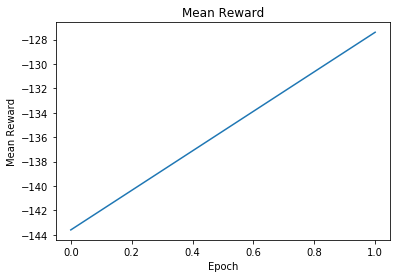
\includegraphics[width=\textwidth]
         	{images/mean_reward_0}
         	\caption{$\pi_0$ mean reward}
         	\label{fig:pi_0_reward}
     	\end{subfigure}
     	\hfill
     	\begin{subfigure}[b]{0.3\textwidth}
         	\centering
         	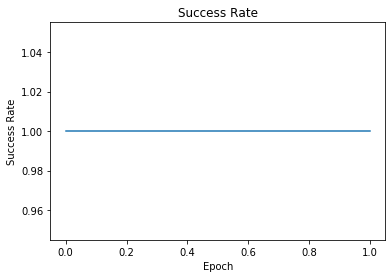
\includegraphics[width=\textwidth]
         	{images/success_rate_0}
         	\caption{$\pi_0$ success rate}
         	\label{fig:pi_0_reward}
     	\end{subfigure}
     	\hfill
     	\begin{subfigure}[b]{0.3\textwidth}
         	\centering
         	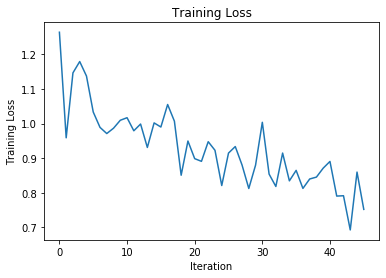
\includegraphics[width=\textwidth]
         	{images/training_loss_0}
         	\caption{$\pi_0$ training loss}
         	\label{fig:pi_0_reward}
     	\end{subfigure}
     	\centering
     	\begin{subfigure}[b]{0.3\textwidth}
         	\centering
         	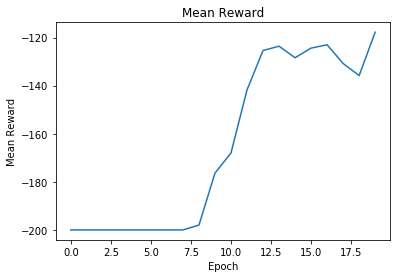
\includegraphics[width=\textwidth]
         	{images/mean_reward_1}
         	\caption{$\pi_1$ mean reward}
         	\label{fig:pi_1_reward}
     	\end{subfigure}
     	\hfill
     	\begin{subfigure}[b]{0.3\textwidth}
         	\centering
         	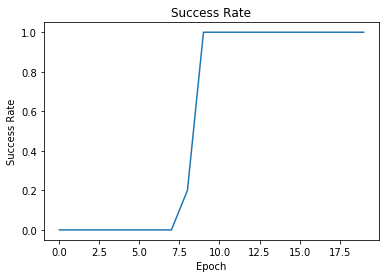
\includegraphics[width=\textwidth]
         	{images/success_rate_1}
         	\caption{$\pi_1$ success rate}
         	\label{fig:pi_1_reward}
     	\end{subfigure}
     	\hfill
     	\begin{subfigure}[b]{0.3\textwidth}
         	\centering
         	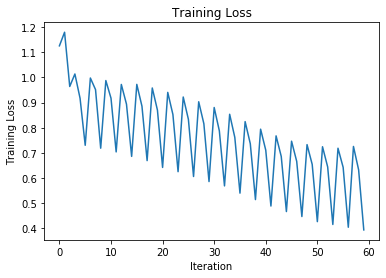
\includegraphics[width=\textwidth]
         	{images/training_loss_1}
         	\caption{$\pi_1$ training loss}
         	\label{fig:pi_1_reward}
     	\end{subfigure}
     	\centering
     	\begin{subfigure}[b]{0.3\textwidth}
         	\centering
         	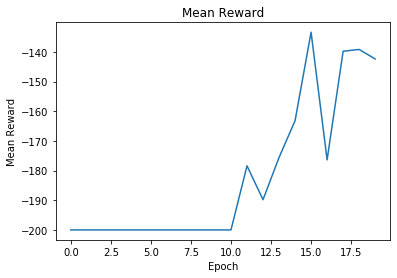
\includegraphics[width=\textwidth]
         	{images/mean_reward_2}
         	\caption{$\pi_2$ mean reward}
         	\label{fig:pi_2_reward}
     	\end{subfigure}
     	\hfill
     	\begin{subfigure}[b]{0.3\textwidth}
         	\centering
         	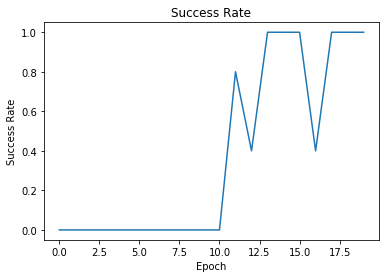
\includegraphics[width=\textwidth]
         	{images/success_rate_2}
         	\caption{$\pi_2$ success rate}
         	\label{fig:pi_2_reward}
     	\end{subfigure}
     	\hfill
     	\begin{subfigure}[b]{0.3\textwidth}
         	\centering
         	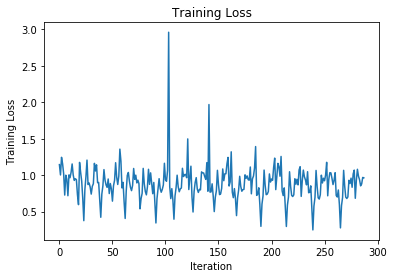
\includegraphics[width=\textwidth]
         	{images/training_loss_2}
         	\caption{$\pi_2$ training loss}
         	\label{fig:pi_2_reward}
     	\end{subfigure}
	\end{figure}
	
	\noindent
	Analysis:\\\\
	1. Mean Reward: For $\pi_0$, the mean reward is a straight line because there are only two epochs so the tests can only be run for two times and the mean reward rises up immediately. In comparison, the mean rewards of $\pi_1$ and $\pi_2$ increase gradually, while the latter one has a larger oscillation. This is because the dataset is changing within every epoch for $\pi_2$.\\\\
	2. Success Rate: The success rate curve for $\pi_0$ remains a line and the rate keeps 100\% after the first epoch. In comparison, the success rates of $\pi_1$ and $\pi_2$ increase to a high level after several epochs, with $\pi_1$ keeping steady and $\pi_2$ occasionally oscillating.\\\\
	3. Training Loss: The training losses of $\pi_0$ and $\pi_1$ goes down gradually, but the second one is oscillating much stronger because only two expert episodes data are feeded into $\pi_1$. On the contrary, the training loss for $\pi_2$ keeps the same level all the time. There are several spikes appearing periodically, indicating that the training loss is decreasing within every epoch, but since the dataset is aggregated in every dagger iteraion, the training loss becomes large again when a new epoch begins.
    
\end{document}